\documentclass[xcolor=dvipsnames]{beamer}
\usepackage{graphicx} % Required for inserting images
\usepackage{bm}

\usepackage{multimedia}
\usepackage{hyperref}


\usetheme{Madrid}
\useinnertheme{circles}

\definecolor{LUT4}{HTML}{23B900} % green
\definecolor{LUT2}{HTML}{000000} % black
\definecolor{LUT3}{HTML}{ff8621} % yellow
\definecolor{LUT1}{HTML}{ed174d}

\setbeamercolor{palette primary}{bg=LUT2,fg=white}
\setbeamercolor{palette secondary}{bg=LUT1,fg=white}
% \setbeamercolor{palette tertiary}{bg=LUT3,fg=white}
% \setbeamercolor{palette quaternary}{bg=LUT4,fg=white}
\setbeamercolor{structure}{fg=LUT2} % itemize, enumerate, etc
\setbeamercolor{section in toc}{fg=LUT2} % TOC sections

% Override palette coloring with secondary
\setbeamercolor{subsection in head/foot}{bg=LUT1}
\setbeamercolor{title in head/foot}{bg=LUT4}
\setbeamercolor{date in head/foot}{bg=LUT3}
\setbeamercolor{author in head/foot}{bg=LUT1}

\logo{
\includegraphics[height=0.8cm]{resources/LUT_logo.png}}

\title[A Case Study on Flappy Bird AI]{What does it take for an AI to beat a score of 100 in Flappy Bird?}
\subtitle{A Case Study on Flappy Bird AI}
\author{Arno Törö}
\date{\today}
\institute[]{LUT University}

\begin{document}

\begin{frame}
    \titlepage
\end{frame}

\begin{frame}
    \tableofcontents
\end{frame}


\section{Introduction}
\begin{frame}{Introduction}
    \begin{itemize}
        \item Flappy Bird was a popular game in 2014 and it became infamous for its simple but challenging gameplay.
    \end{itemize}
    \begin{center}
        \vspace{0.3cm} % Additional vertical space
        
\includegraphics[width=0.8\textwidth]{resources/flappy_bird.png}
    \end{center}
\end{frame}

\begin{frame}{Introduction}
    \begin{itemize}
        \item The motivation for this case study was to have an intuitive but relatively simple problem and try to develop an AI agent to solve it.
        \item The agent is trained in the game environment through trial and error, using a reinforcement learning algorithm called deep Q-learning algorithm.
    \end{itemize}
\end{frame}




\section{Methodology}
\begin{frame}{Environment setup}
    \begin{itemize}
        \item Created a game environment of Flappy Bird in Python, which handles the game logic (collisions, rendering more pipes, etc.).
        \item There are two possible actions in the game: flap or don't flap
        \item Return the game state information of each frame to the agent.
    \end{itemize}
\end{frame}

\begin{frame}{Information to agent}
    \begin{itemize}
        \item Information gathered for the agent:
        \begin{enumerate}
            \item Horizontal distance to next pipe
            \item Vertical distance to next center of pipe gap
            \item Bird's current speed
        \end{enumerate}
    \end{itemize}
    \begin{center}
        \vspace{0.05cm} % Additional vertical space
        
\includegraphics[width=0.7\textwidth]{resources/flappy_bird_game_state.png}
    \end{center}
\end{frame}

\begin{frame}{Deep Q-learning algorithm}
    \begin{itemize}
        \item Utilized PyTorch
        \item Q-learning calculates a value for each possible action in a state.
        \item Deep Q-learning (DQN) uses neural networks to approximate Q-values for each possible action at given state.
        \item DQNs often utilize CNNs to approximate Q-values, but not used in this study. 
        \item \(\epsilon\)-greedy policy
        \begin{itemize}
            \item Balance exploration and exploitation to prevent suboptimal results
        \end{itemize}
        \begin{center}
            \vspace{0.05cm} % Additional vertical space
            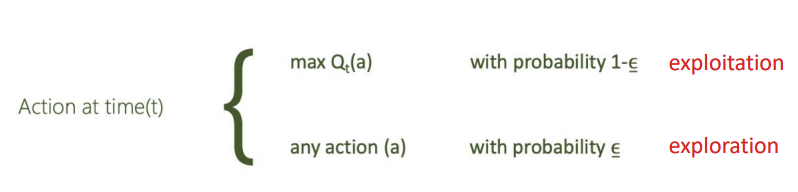
\includegraphics[width=0.7\textwidth]{resources/epsilon_greedy.png}
        \end{center}
    \end{itemize}
\end{frame}


\begin{frame}{Deep Q-learning algorithm structure}
    \begin{center}
        \vspace{0.05cm} % Additional vertical space
        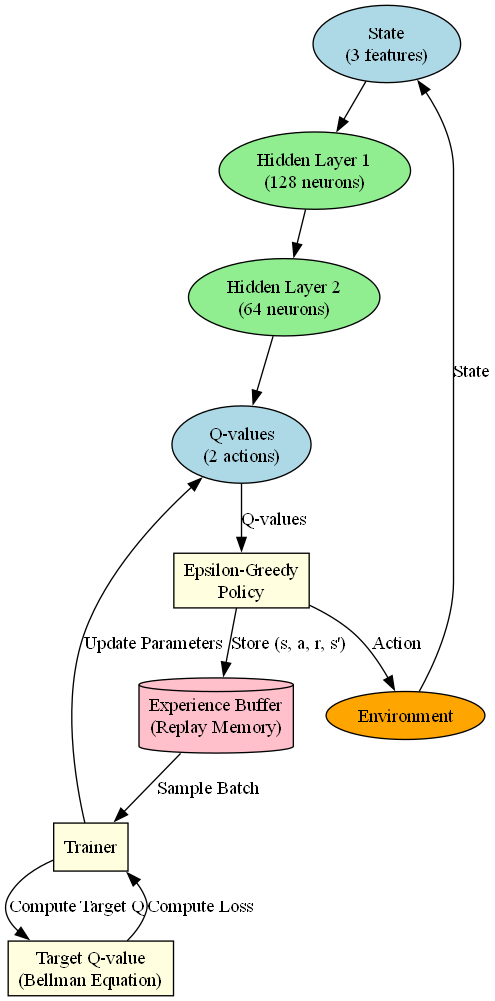
\includegraphics[height=0.65\textwidth]{resources/dqn_architecture_diagram.png}
    \end{center}
\end{frame}


\begin{frame}{Used hyperparameters}
    \begin{itemize}
        \item Hyperparameters used in this study
        \begin{itemize}
            \item Learning rate: 0.001
            \item \(\gamma\): 0.95
            \item Batch size: 128
            \item Replay buffer size: 20 000
            \item \(\epsilon\): decay form 1.0 to 0.1 over time.
        \end{itemize}
        \item Rewards given for the agent:
        \begin{itemize}
            \item Surviving: 0.01
            \item Passing a pipe: 1
            \item Failing: -10
        \end{itemize}
    \end{itemize}
\end{frame}

\section{Results}
\begin{frame}{Results}
    \begin{itemize}
        \item Agent was trained for 250 iterations or until a score of 200 was achieved with two consecutive games.
        \item Training results of 10 agents:
    \end{itemize}
    \vspace{-0.3cm}
    \begin{table}[h!]
        % \caption{Training results: Iterations required for the agent to reach 100 points or fail (i.e., 250 iterations).}
        % \label{tab:training_results}
        \centering
        \small
        \begin{tabular}{|l|r|}
            \hline
            \textbf{Training Session} & \textbf{Iterations to Reach Goal or Fail} \\
            \hline
            1 & 99 \\
            2 & 250 \\
            3 & 250 \\
            4 & 90 \\
            5 & 250 \\
            6 & 250 \\
            7 & 105 \\
            8 & 95 \\
            9 & 94 \\
            10 & 97 \\
            \hline
            Average & 158 \\
            \hline
        \end{tabular}
    \end{table}

\end{frame}


\begin{frame}{Training session performance}
    \begin{itemize}
        \item Agent's performance on one training session which lead to reaching a score of 100 points
    \end{itemize}
    \begin{center}
        \vspace{0.05cm} % Additional vertical space
        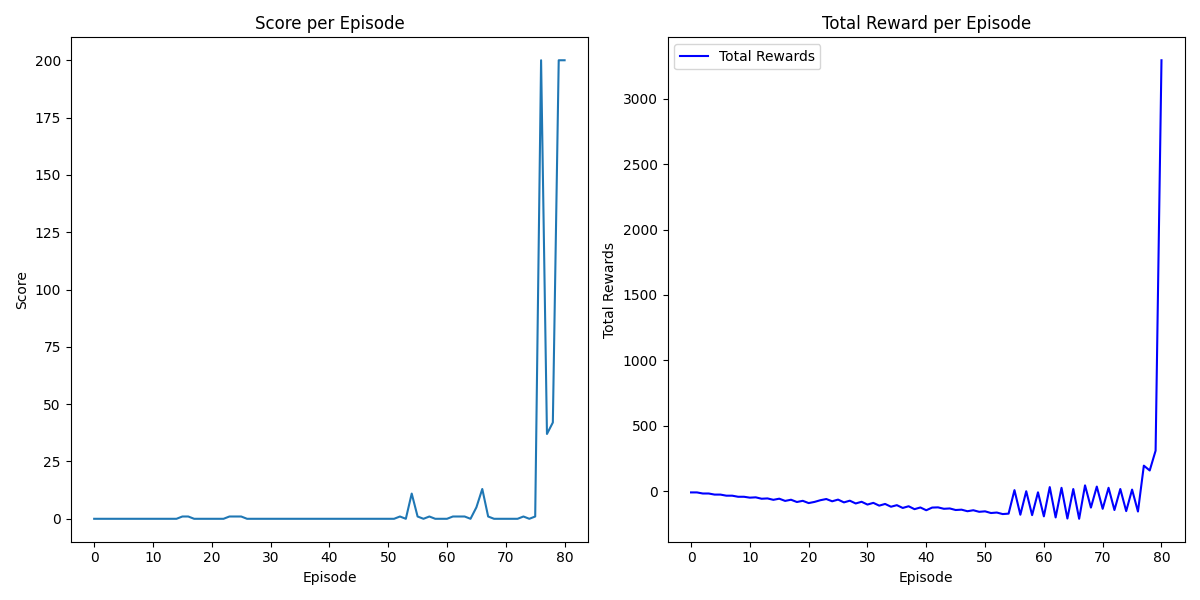
\includegraphics[height=0.5\textwidth, width=\textwidth]{resources/figure1.png}
    \end{center}
\end{frame}


\section{Conclusion}
\begin{frame}{Conclusions}
    \begin{itemize}
        \item Agent is capable of reaching 100 points of score rather quickly.
        \item Sometimes fails to converge to a solution, the first pipe pass is the most important one. Can be based on luck.
        \item Improvements in hyperparameters or learning algorithm structure could help overcome this issue.
    \end{itemize}
\end{frame}

\begin{frame}{Demovideo}

\end{frame}


\end{document}
